% begin module optimization-ex1
\begin{frame}
\begin{example}[Example 1, p. 257]
\alert<handout:0| 10>{A farmer has 2400 ft of fencing} and wants to fence off a rectangular field that borders a straight river.  He doesn't need to put fencing along the river.  What are the dimensions of the field with the largest area?
\begin{columns}[c]
\column{.5\textwidth}
\ \only<handout:0| -2>{%
\uncover<2>{%
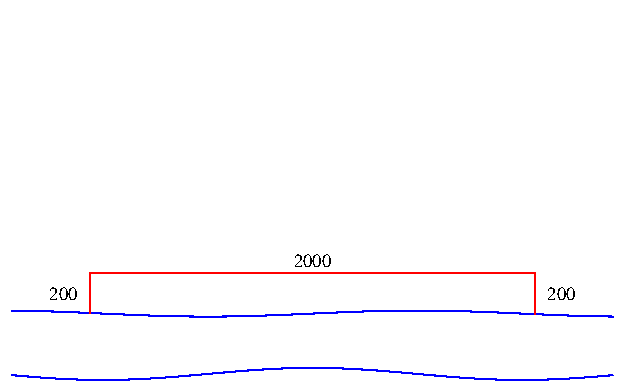
\includegraphics[width=5cm]{optimization/pictures/04-07-ex1a.pdf}%
}}%
\only<handout:0| 3>{%
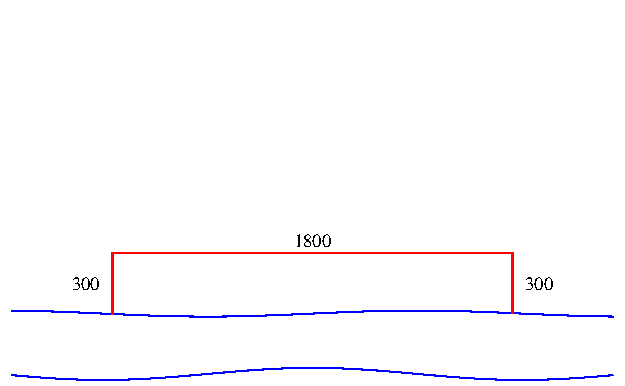
\includegraphics[width=5cm]{optimization/pictures/04-07-ex1b.pdf}%
}%
\only<handout:0| 4>{%
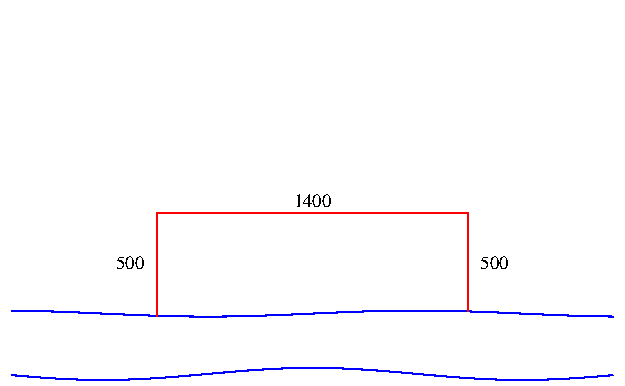
\includegraphics[width=5cm]{optimization/pictures/04-07-ex1c.pdf}%
}%
\only<handout:0| 5>{%
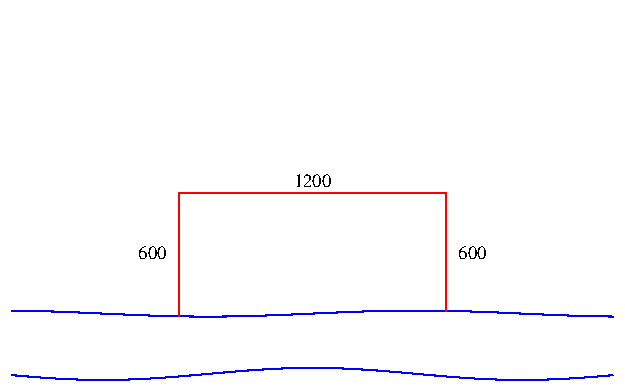
\includegraphics[width=5cm]{optimization/pictures/04-07-ex1d.pdf}%
}%
\only<handout:0| 6>{%
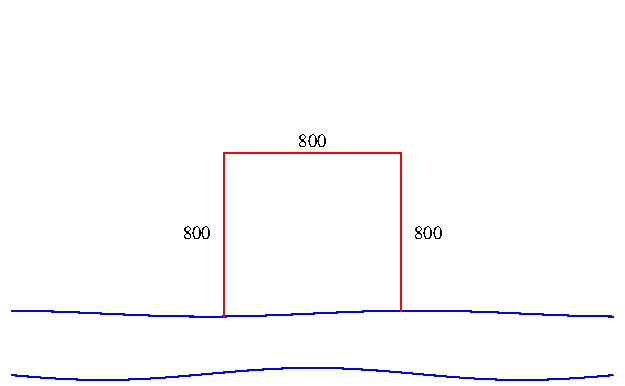
\includegraphics[width=5cm]{optimization/pictures/04-07-ex1e.pdf}%
}%
\only<handout:0| 7>{%
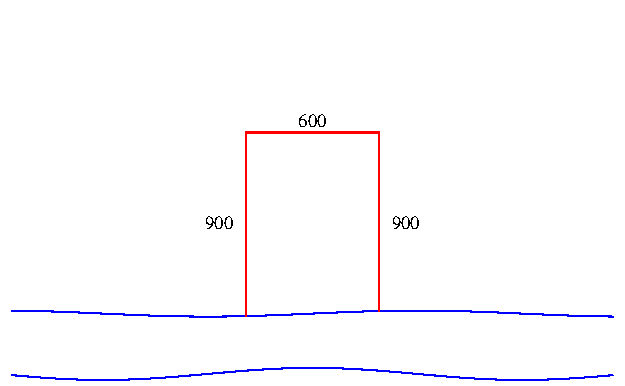
\includegraphics[width=5cm]{optimization/pictures/04-07-ex1f.pdf}%
}%
\only<handout:0| 8>{%
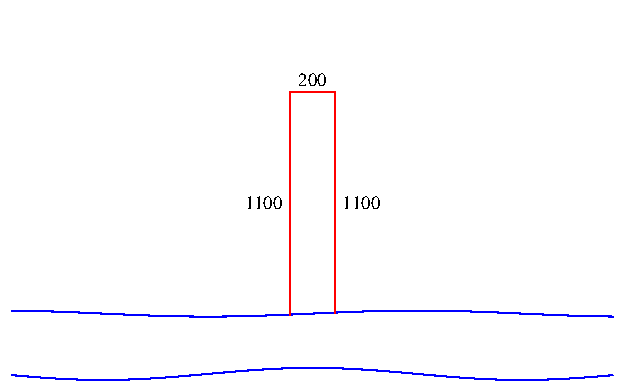
\includegraphics[width=5cm]{optimization/pictures/04-07-ex1g.pdf}%
}%
\only<9->{%
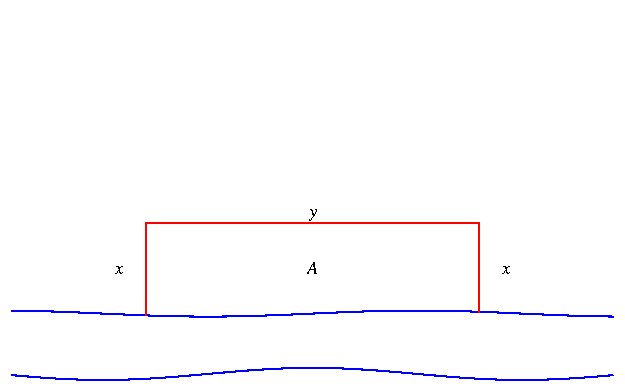
\includegraphics[width=5cm]{optimization/pictures/04-07-ex1h.pdf}%
}%

\uncover<2->{%
Area $ = %
\only<9->{%
A = xy
}%
\only<handout:0| -8>{%
\only<handout:0| -2>{200}%
\only<handout:0| 3>{300}%
\only<handout:0| 4>{500}%
\only<handout:0| 5>{600}%
\only<handout:0| 6>{800}%
\only<handout:0| 7>{900}%
\only<handout:0| 8>{1100}%
\cdot%
 \only<handout:0| -2>{2000} %
\only<handout:0| 3>{1800}%
\only<handout:0| 4>{1400}%
\only<handout:0| 5>{1200}%
\only<handout:0| 6>{800}%
\only<handout:0| 7>{600}%
\only<handout:0| 8>{200}%
= %
\only<handout:0| -2>{400,000}%
\only<handout:0| 3,7>{540,000}%
\only<handout:0| 4>{700,000}%
\only<handout:0| 5>{720,000}%
\only<handout:0| 6>{640,000}%
\only<handout:0| 8>{220,000}%
}$\only<handout:0| -8>{ft$^2$}
}%
\uncover<20->{%
\abovedisplayskip=0pt
\belowdisplayskip=0pt
\[
\begin{array}{r|r}
x & A(x)\\
\hline
\alert<handout:0| 21-22>{0} & \alert<handout:0| 22>{\uncover<22->{0}}\\
\alert<handout:0| 23-24,27>{600} & \alert<handout:0| 24,27>{\uncover<24->{720,000}}\\
\alert<handout:0| 25-26>{1200} & \uncover<26->{\alert<handout:0| 26>{0}}
\end{array}
\]
}%
\column{.5\textwidth}
\uncover<9->{%
Let $x$ and $y$ denote the depth and width of the rectangle (in feet).  Let $A$ be its area.%
}%
\abovedisplayskip=0pt
\belowdisplayskip=0pt
\begin{eqnarray*}
\uncover<10->{2x + y} & \uncover<10->{=} & \uncover<10->{2400}\\
\uncover<11->{\alert<handout:0| 13>{y}} & \uncover<11->{\alert<handout:0| 13>{=}} & \uncover<11->{\alert<handout:0| 13>{2400 - 2x}}
\end{eqnarray*}
\abovedisplayskip=0pt
\belowdisplayskip=0pt
\begin{eqnarray*}
\uncover<12->{A} & \uncover<12->{=} & \uncover<12->{x\alert<handout:0| 13>{y}} \uncover<13->{=  x(\alert<handout:0| 13>{2400-2x})}\\
& \uncover<14->{=} & \uncover<14->{2400x - 2x^2}%
\end{eqnarray*}
\uncover<15->{Notice that $0\leq x \leq 1200$.}

\uncover<16->{%
Maximize the function $A(x)$:
\[
\alert<handout:0| 16-17>{A'(x) = \uncover<17->{2400 - 4x}}%
\]
}%
\uncover<18->{%
Critical number: \alert<handout:0| 18-19>{$x = $ \uncover<19->{$600$.}} 
}%
\end{columns}
\uncover<27->{%
Therefore the maximum area occurs when $x = 600$ft and $y = 1200$ft.
}%
\end{example}
\end{frame}
% end module optimization-ex1
